\documentclass{article}
\usepackage{cmap}
\usepackage[utf8]{inputenc}
\usepackage[english,ukrainian]{babel}
\usepackage{graphicx}
\usepackage{geometry}
\usepackage{listings}
\usepackage{float}
\usepackage{amsmath}
\geometry{
	a4paper,
	left=20mm,
	right=20mm,
	top=15mm,
	bottom=15mm,
}
\lstset{
	language=c,
	tabsize=4,
	keepspaces,
	showstringspaces=false,
}
\graphicspath{ {./pictures} }
\setlength{\parindent}{4em}

\newcommand\subject{Організація комп’ютерних мереж}
\newcommand\lecturer{асистент кафедри ПЗ \\ Задорожний І.М.}
\newcommand\teacher{асистент кафедри ПЗ \\ Задорожний І.М.}
\newcommand\mygroup{ПЗ-22}
\newcommand\lab{5}
\newcommand\theme{Дослідження протоколів SMTP і POP3}
\newcommand\purpose{Ознайомитися зі службою електронної пошти та основними командами протоколів SMTP і POP3 і навчитися користуватися утилітою telnet для зв’язку з серверами вхідної та вихідної пошти}

\begin{document}
\begin{normalsize}
	\begin{titlepage}
		\thispagestyle{empty}
		\begin{center}
			\textbf{МІНІСТЕРСТВО ОСВІТИ І НАУКИ УКРАЇНИ\\
				НАЦІОНАЛЬНИЙ УНІВЕРСИТЕТ "ЛЬВІВСЬКА ПОЛІТЕХНІКА"}
		\end{center}
		\begin{flushright}
			\textbf{ІКНІ}\\
			Кафедра \textbf{ПЗ}
		\end{flushright}
		\vspace{200pt}
		\begin{center}
			\textbf{ЗВІТ}\\
			\vspace{10pt}
			до лабораторної роботи № \lab\\
			\textbf{на тему}: “\textit{\theme}”\\
			\textbf{з дисципліни}: “\subject”
		\end{center}
		\vspace{112pt}
		\begin{flushright}
			
			\textbf{Лектор}:\\
			\lecturer\\
			\vspace{28pt}
			\textbf{Виконав}:\\
			
			студент групи \mygroup\\
			Коваленко Д.М.\\
			\vspace{28pt}
			\textbf{Прийняв}:\\
			
			\teacher\\
			
			\vspace{28pt}
			«\rule{1cm}{0.15mm}» \rule{1.5cm}{0.15mm} 2023 р.\\
			$\sum$ = \rule{1cm}{0.15mm}……………\\
			
		\end{flushright}
		\vspace{\fill}
		\begin{center}
			\textbf{Львів — 2023}
		\end{center}
	\end{titlepage}
		
	\begin{description}
		\item[Тема.] \theme.
		\item[Мета.] \purpose.
	\end{description}

\section*{Теоретичні відомості}
SMTP (Simple Mail Transfer Protocol, Простий протокол пересилання пошти) – протокол прикладного рівня, призначений для пересилання електронної пошти до поштового сервера з клієнта-комп’ютера або між поштовими серверами. Опис SMTP даний у RFC 821 і 1123. Зараз на практиці використовується розширений SMTP (Extended SMTP, ESMTP), опис якого даний у RFC 2821.

Telnet (Terminal NETwork) мережевий протокол для реалізації текстового інтерфейсу в мережі і назва утиліти, що реалізує клієнтську частину протоколу. Запускається з командного рядка. Використовує 23 порт TCP/UDP.

Протокол POP існує у трьох версіях – POP, POP2 і POP3 (всі вони різні і несумісні між собою), проте версії POP і POP2 застаріли, “на арені” лишився протокол POP3. Протокол IMAP теж має ряд версій. Усі листи кожного користувача зберігаються у окремому місці на диску поштового сервера. Коли користувач перевіряє пошту за протоколом IMAP, завантажуються лише заголовки повідомлень, а ціле повідомлення почне завантажуватися з сервера тоді, коли користувач вибере його заголовок. Натомість протокол POP3 передбачає завантаження цілих повідомлень одразу. 

POP3 – версія протоколу POP (Post Office Protocol, протокол доставки пошти), що відповідає за доставку листів користувачеві з поштового сервера та видалення пошти з сервера. А саме, за протоколом POP3 користувач може звернутися до поштового сервера, на диску якого зберігається його кореспонденція (ця область пам’яті і є поштовою скринькою) та зчитати звідти листи. Доступ до POP3-сервера можна отримати з довільної точки Інтернету. POP3 визначений у RFC 1225.


\section*{Хід виконання}
\begin{figure}[H]
	\centering
	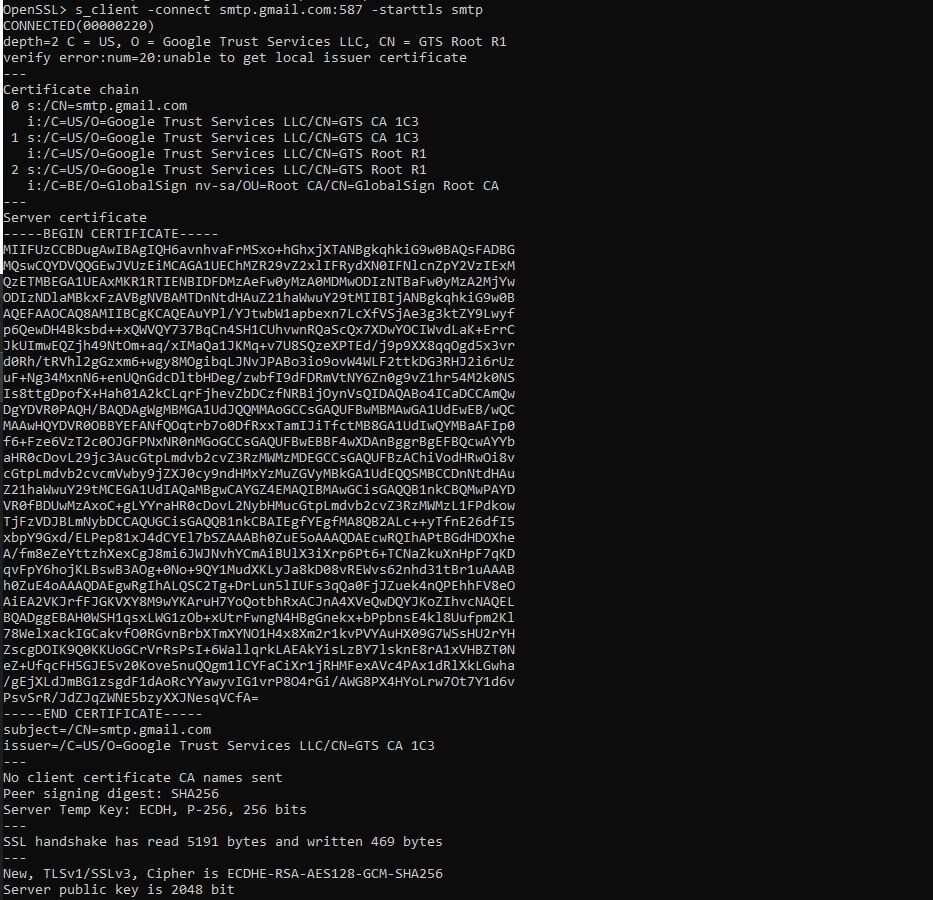
\includegraphics[width=\textwidth]{11}
\end{figure}
\begin{figure}[H]
	\centering
	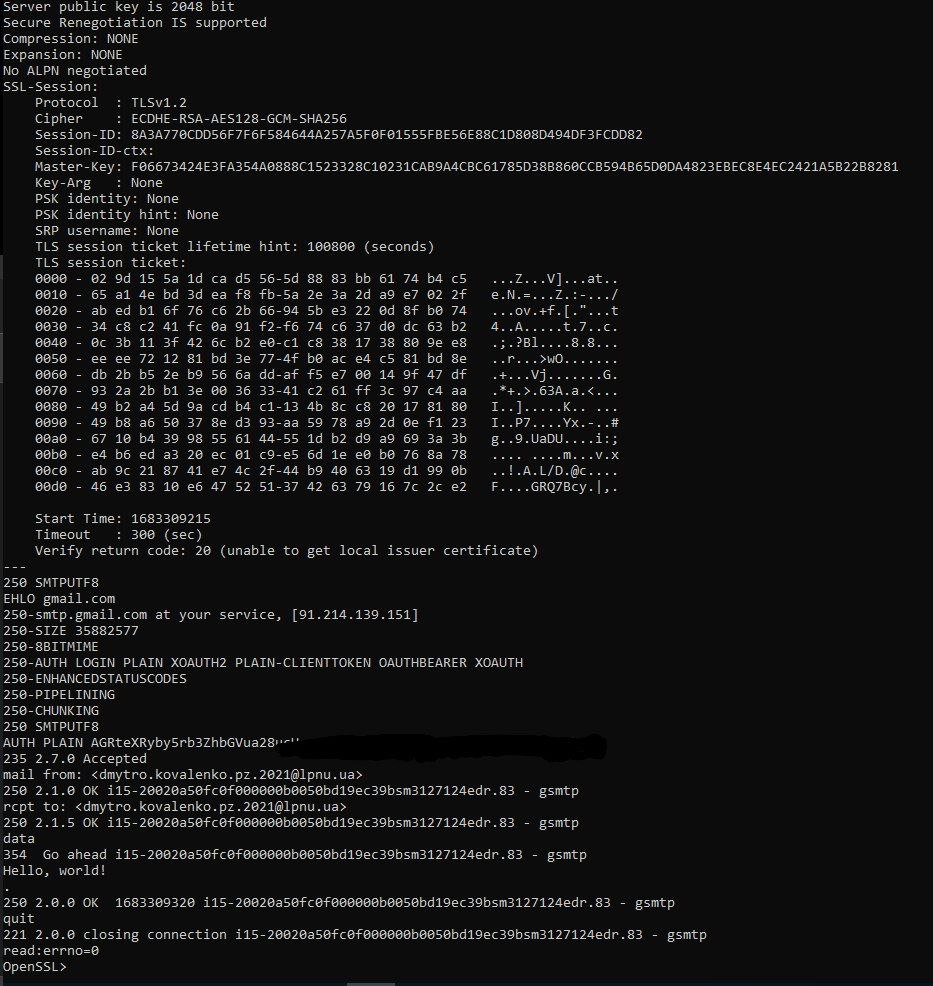
\includegraphics[width=\textwidth]{12}
\end{figure}
\begin{figure}[H]
	\centering
	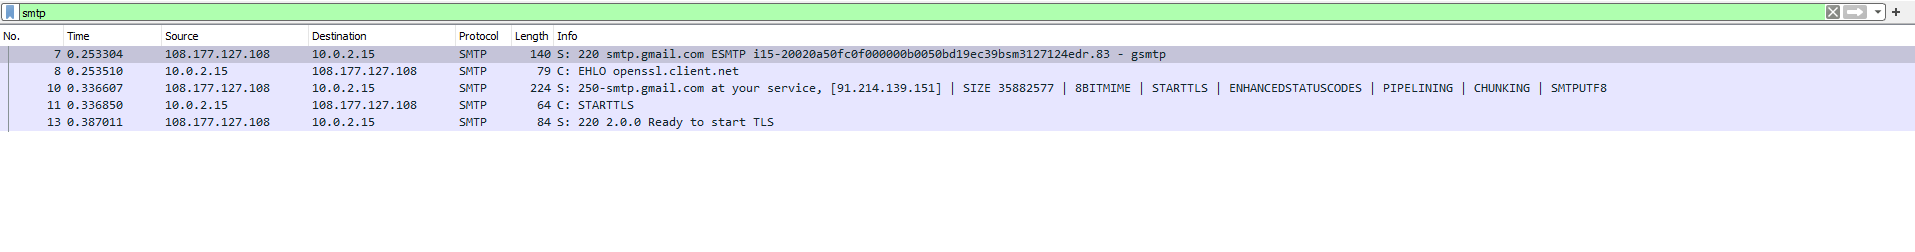
\includegraphics[width=\textwidth]{13}
\end{figure}
\begin{figure}[H]
	\centering
	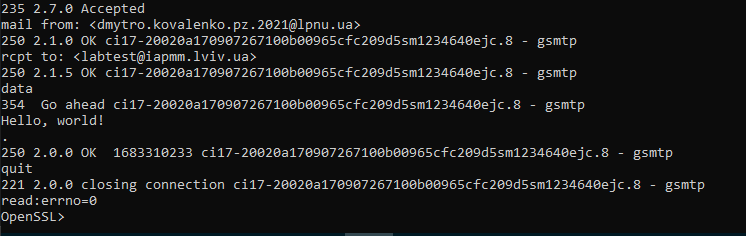
\includegraphics[width=\textwidth]{15}
\end{figure}
\begin{figure}[H]
	\centering
	
\includegraphics[width=\textwidth]{14}
\end{figure}
\begin{figure}[H]
	\centering
	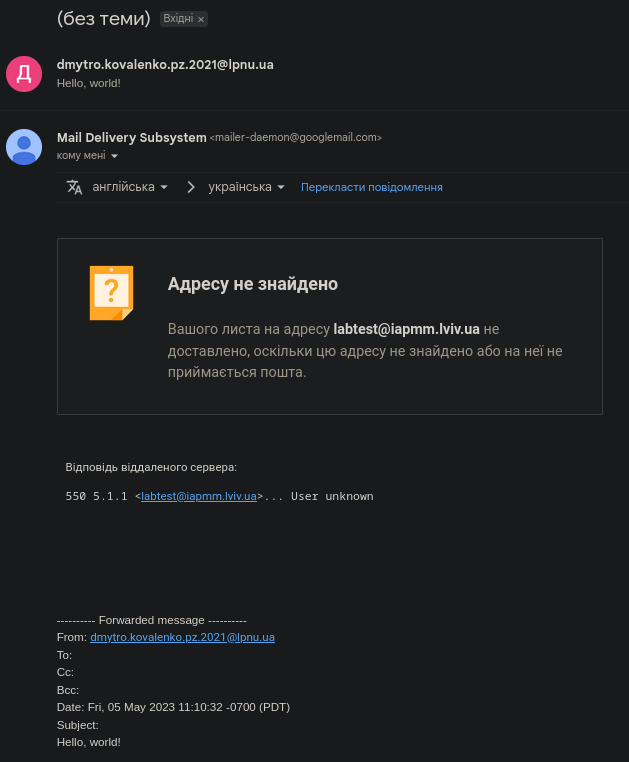
\includegraphics[width=\textwidth]{16}
\end{figure}

\begin{figure}[H]
	\centering
	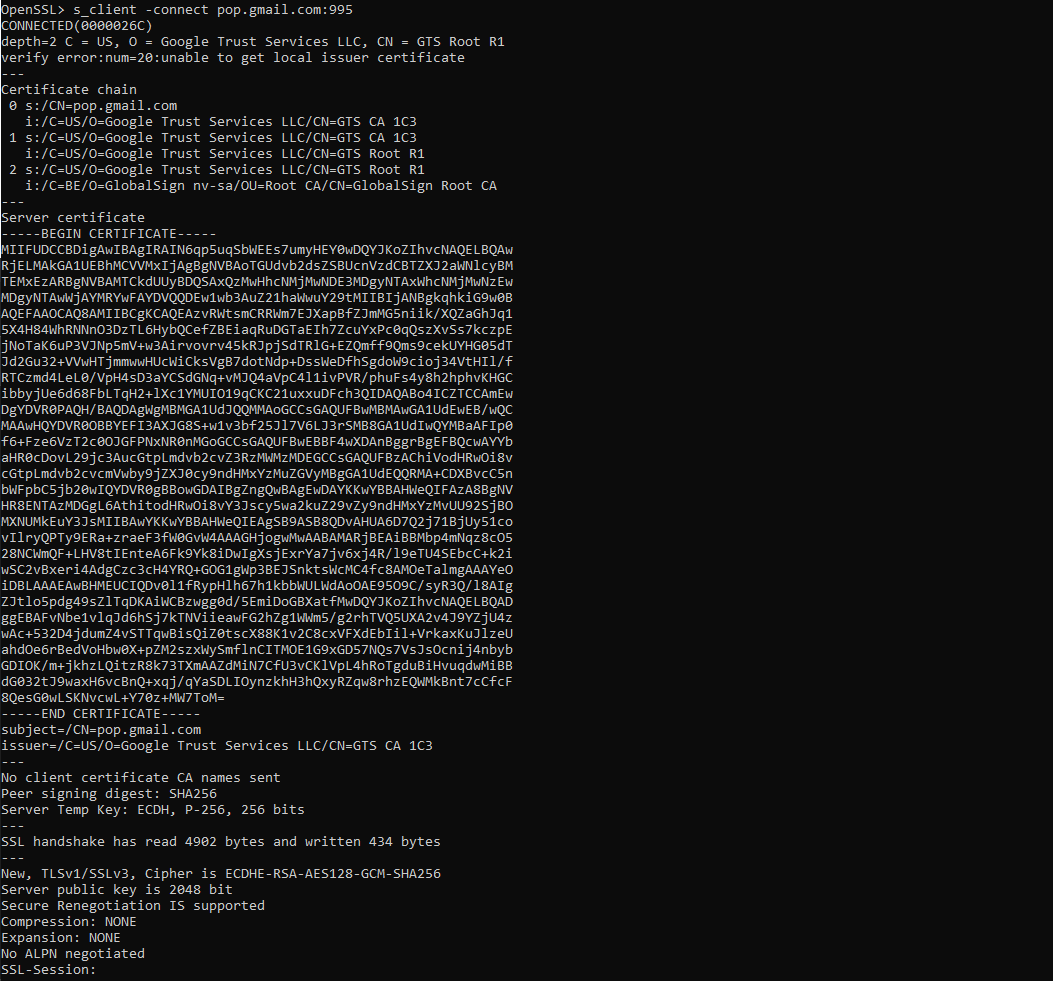
\includegraphics[width=\textwidth]{21}
\end{figure}
\begin{figure}[H]
	\centering
	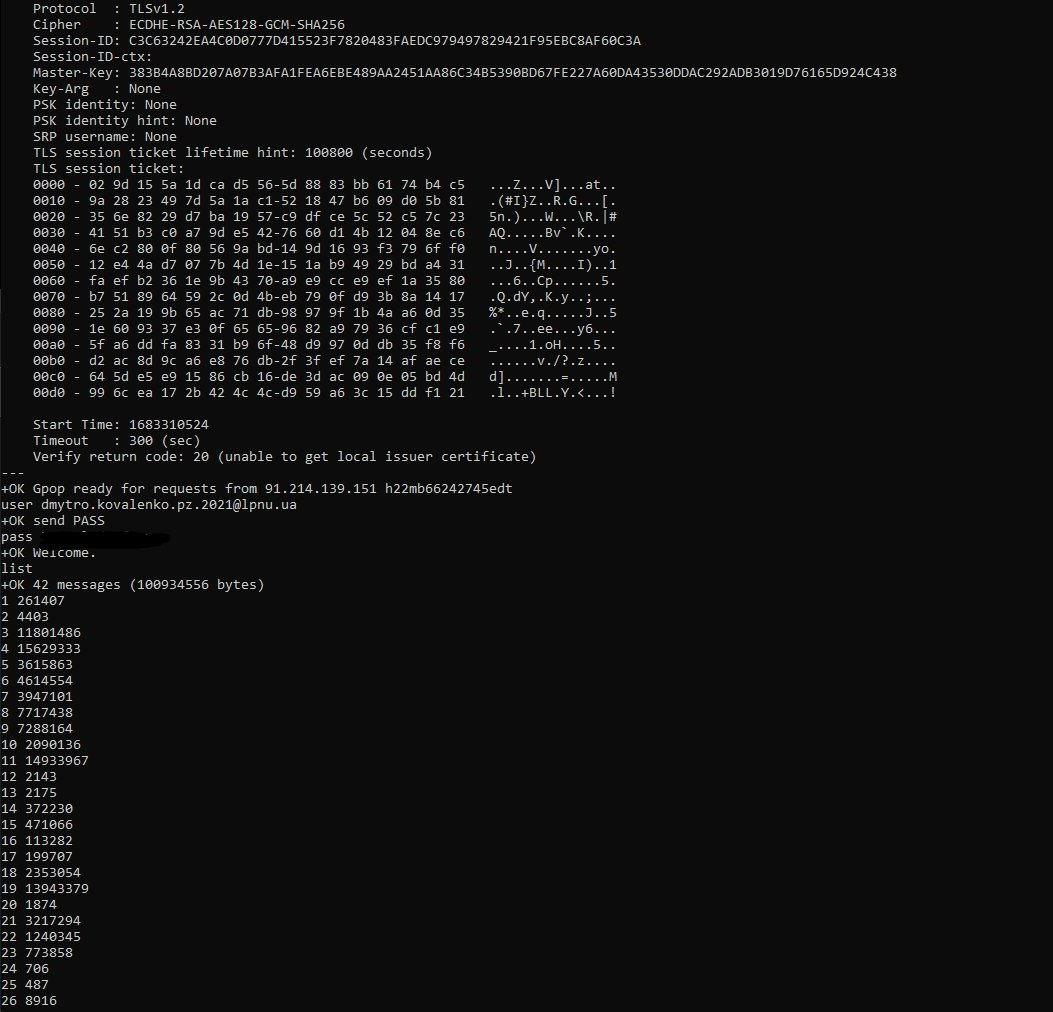
\includegraphics[width=\textwidth]{22}
\end{figure}
\begin{figure}[H]
	\centering
	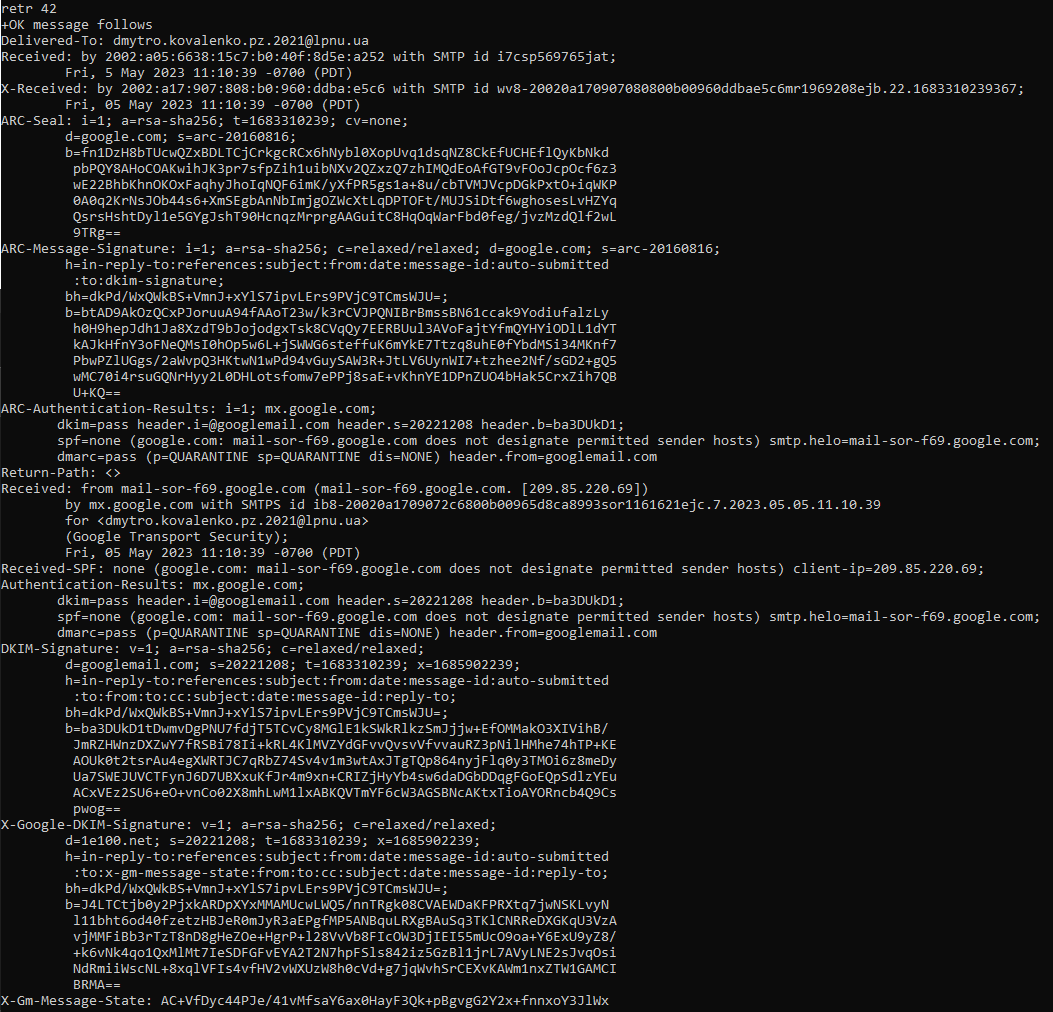
\includegraphics[width=\textwidth]{23}
	\caption{Читання листа 1/4}
\end{figure}
\begin{figure}[H]
	\centering
	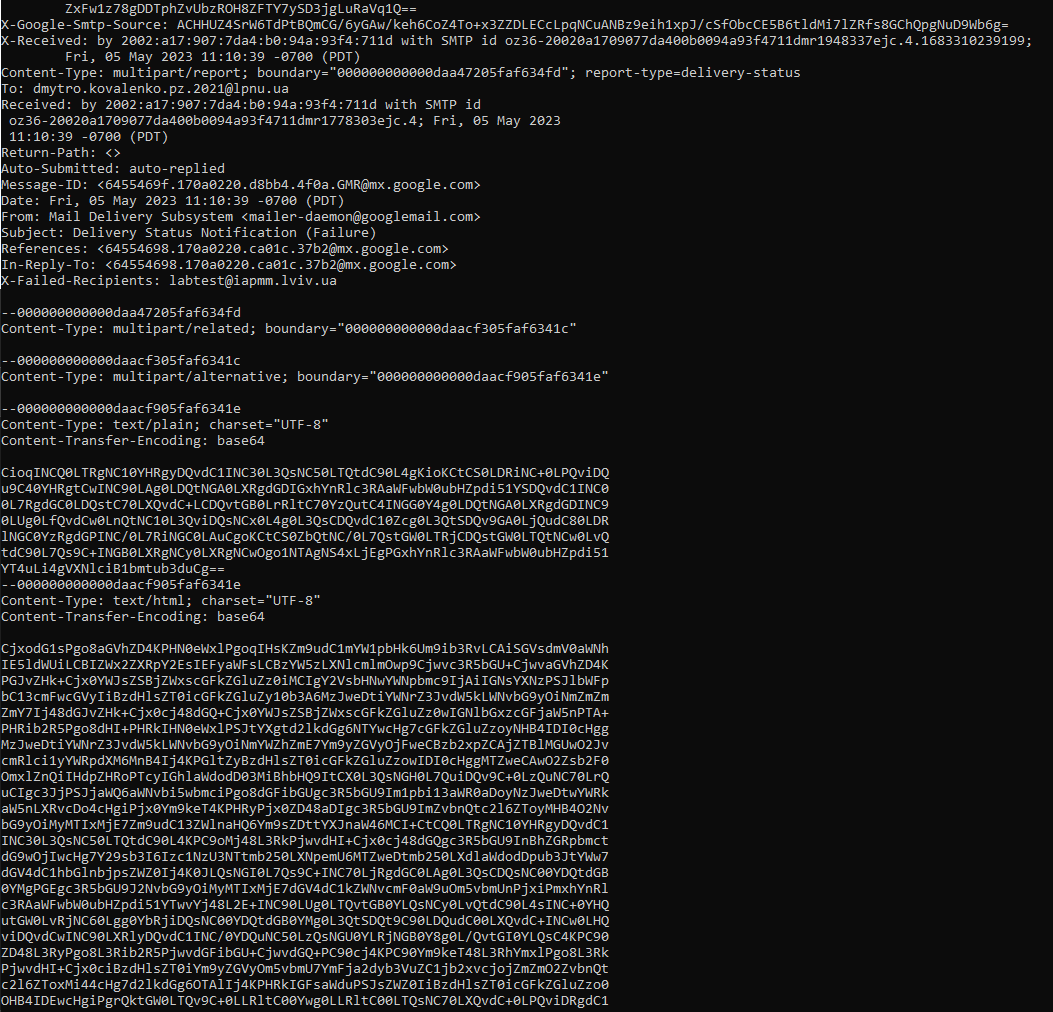
\includegraphics[width=\textwidth]{24}
	\caption{Читання листа 2/4}
\end{figure}
\begin{figure}[H]
	\centering
	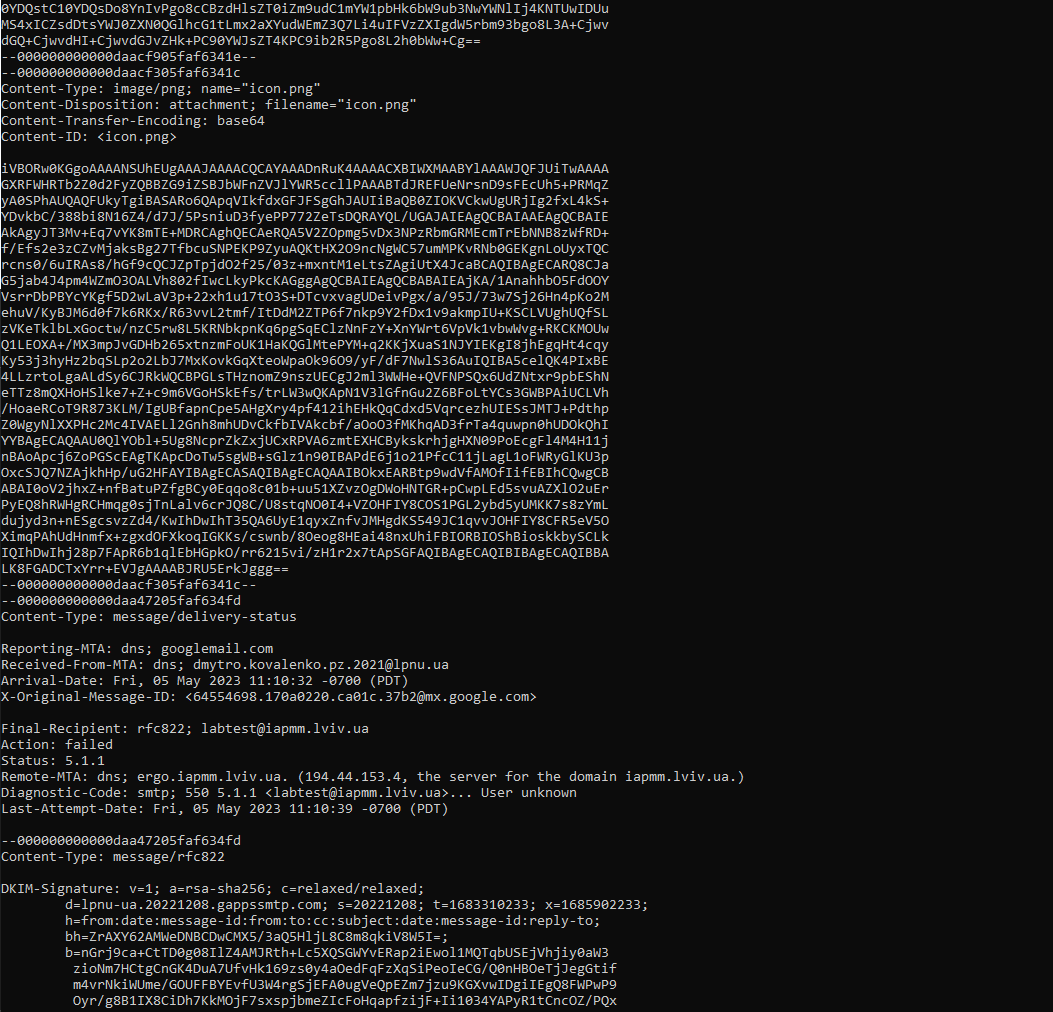
\includegraphics[width=\textwidth]{25}
	\caption{Читання листа 3/4}
\end{figure}
\begin{figure}[H]
	\centering
	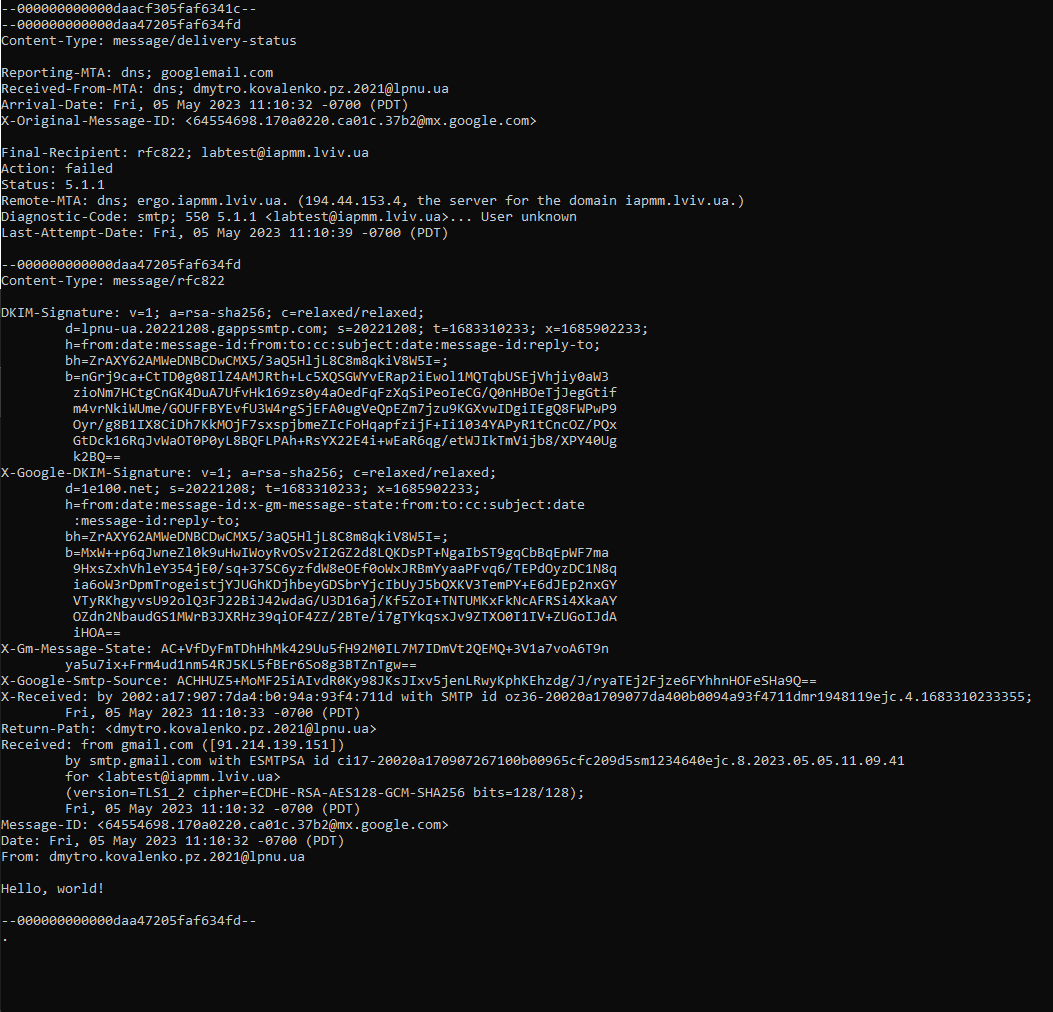
\includegraphics[width=\textwidth]{26}
	\caption{Читання листа 4/4}
\end{figure}

\begin{figure}[H]
	\centering
	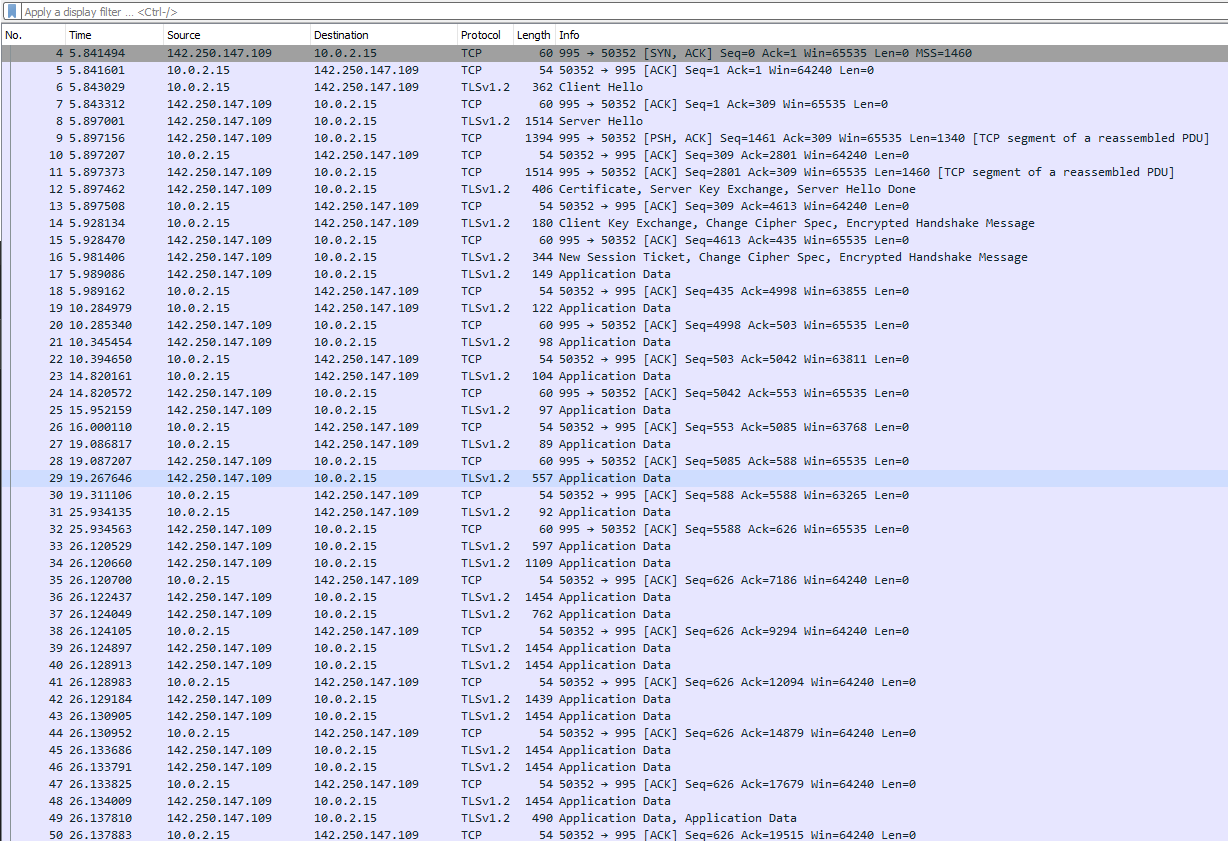
\includegraphics[width=\textwidth]{31}
	\caption{Пакети перехоплені Wireshark під час читання пошти}
\end{figure}

У форматі повідомлення SMTP заголовок From зазвичай містить адресу електронної пошти відправника повідомлення. Він з'являється на початку повідомлення і має наступний формат:

From: електронна-адреса-відправника

Наприклад:

From: john@example.com

Цей заголовок дозволяє отримувачеві знати, хто відправив повідомлення, і зв'язатися з ним у разі необхідності. Крім того, він також допомагає уникнути спаму, оскільки спамери часто використовують неправильні або вигадані адреси відправників.

\section*{Висновки}
Під час виконання лабораторної роботи я ознайомився зі службою електронної пошти та основними командами протоколів SMTP і POP3 і навчився користуватися утилітою telnet для зв’язку з серверами вхідної та вихідної пошти.
	    
\end{normalsize}
\end{document}
